
\section{(R) Airspace Classification}\label{sec:AirspaceClassification}
\paragraph{Motivation:} The \emph{Airspace Classification}, last changed by ICAO in 1990, is described in \cite{icaoAnnex11}. The \emph purpose of airspace classification from \emph{collision avoidance perspective} are following:

\begin{enumerate}
    \item \emph{Separation} - Maintaining a minimum distance between an aircraft and another aircraft or terrain to avoid collisions. There are following separation types:
    \begin{enumerate}[a.]
        \item \emph{Vertical separation} - to ensure that \emph{airspace attendants} are separated by sufficient altitude differences from threats.
        
        \item \emph{Horizontal  separation} - to endure that \emph{airspace attendants} have sufficient horizontal distance from threats
    \end{enumerate}
    
    \item{Clearance} - permission award process by Air Traffic Control (ATC) for an airspace attendant to proceed with flight plan execution/change.
    
    \item \emph{Organization} - ensure that \emph{airspace attendant} can expect minimal level of separation and airspace organization depending on the type.
\end{enumerate}

\begin{note}
    This works focus on \emph{separation} in both controlled/non-controlled airspace.
\end{note}

\paragraph{Airspace Categorization:} The airspace is segmented depending on the \emph{altitude}. The altitude boundaries can be given in the one of two ways:

\begin{enumerate}
    \item \emph{Altitude above Mean Sea Level} (AMSL) - the barometric altitude is used as boundary reference.
    
    \item \emph{Altitude above Ground Level} (AGL) - the boundary copies terrain.
\end{enumerate}

\noindent There is an example of airspace classification for \emph{Australia}\footnote{Australian airspace classification: \url{http://www.airservicesaustralia.com/services/how-air-traffic-control-works/how-airspace-is-managed/}} and \emph{Czech Republic}\footnote{Czech Republic Airspace Classification:\url{https://lis.rlp.cz/vfrmanual/actual/enr_1_en.html}}:


\begin{figure}[H]
	\centering
	\begin{subfigure}{0.44\textwidth}
		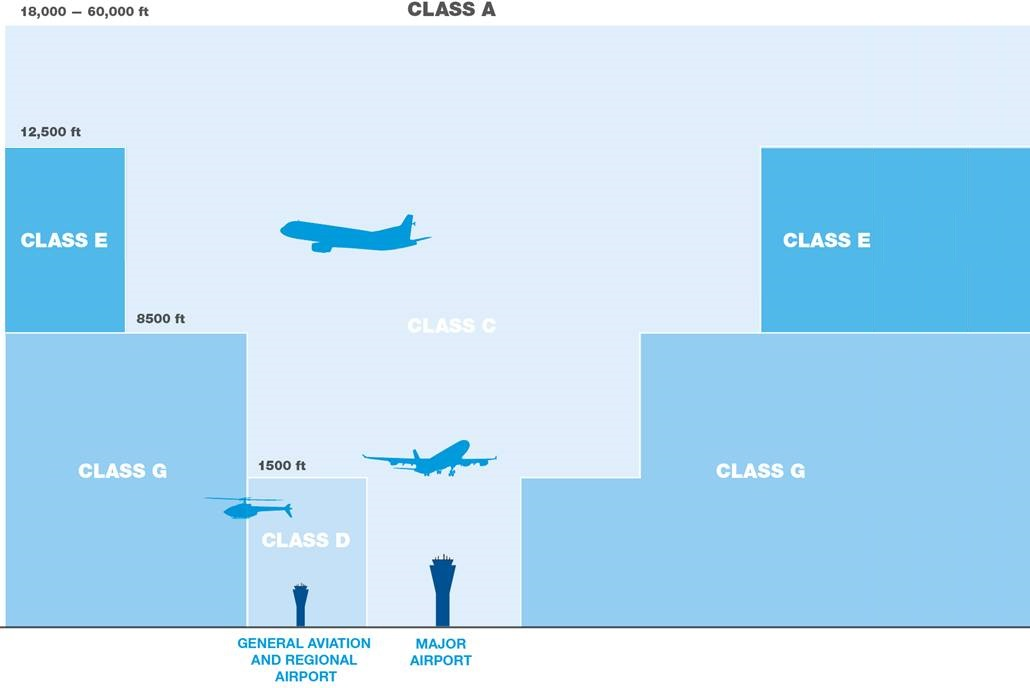
\includegraphics[width=\textwidth]{\FIGDIR/TE055GenericAirspaceClasses}
		\caption{Australian airspace classification.} 
	\end{subfigure}
	\vspace{1em} 
	\begin{subfigure}{0.48\textwidth} % width of right subfigure
		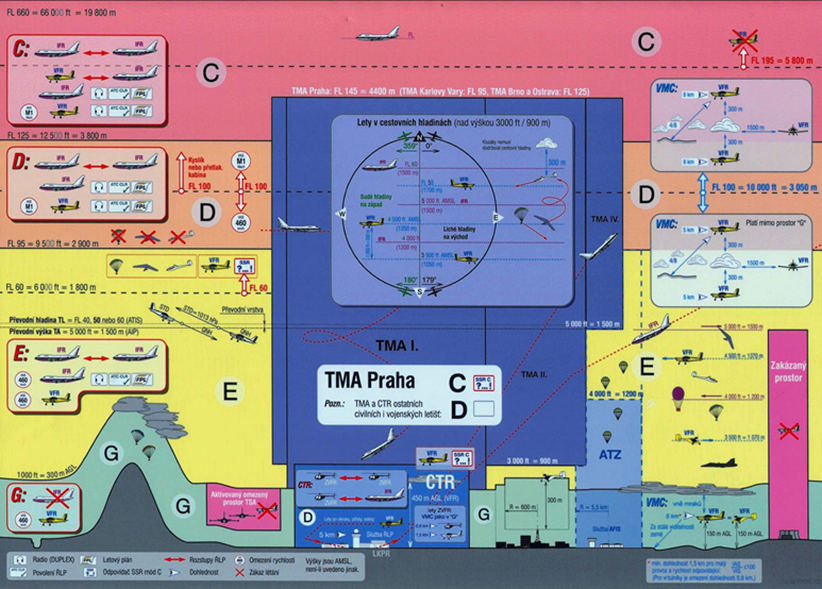
\includegraphics[width=\textwidth]{\FIGDIR/TE056CzechAirspaceClassification}
		\caption{Czech Republic airspace classification.} % subcaption
	\end{subfigure}
	\caption{Airspace classification examples.} % caption for whole figure
\end{figure}

\noindent The \emph{Airspace classes are given like follow}:
\begin{enumerate}
    \item[\textbf{Class A}] \emph{(Upper) Operational Airspace} (18 000 - 60 000 feet AMSL) (considered as part of national airport controlled airspace in EU) - the operational airspace where the most of the commercial/military flights are conducted
    
    \item[\textbf{Class B}] \emph{International Airport Airspace} (0 - 18 000 feet AMSL) (special class of airports in U.S., considered as C airspace in EU) - the airspace down to the ground, with stricter preventive measures against mid-air collision and ground collisions.
    
    \item[\textbf{Class C}] \emph{National Airport Airspace} (0 - 18 000 feet AMSL) - the standard  national level airport airspace with preventive measurements against mid air collision and ground collision situations.
    
    \item[\textbf{Class D}] \emph{Regional Airport Airspace} (0 - 1 500 feet AMSL) - the \emph{regional airport authority} inactive for the most of the time.
    
    \item[\textbf{Class E}] \emph{(Lower) Operational Airspace} (1 500 - 12 500 feet AMSL) - the controlled airspace on lower flight levels, lower airworthiness requirements are applied.
    
    \item[\textbf{Class F}] \emph{(Upper) Uncontrolled Airspace} (500 - 1 500 feet AGL) - the upper portion of uncontrolled airspace (deprecated and merged into E class airspace in most of countries).
    
    \item[\textbf{Class G}] \emph{(Lower) Uncontrolled Airspace} (0 - 500 feet AGL) - the lower portion of \emph{airspace} which is \emph{free to fly}.
\end{enumerate}

\begin{note}
    The \emph{boundaries of the airspace classes} may vary between countries in all segments. The \emph{ATC authority} is usually enforced from \emph{FL-60} (6 000 feet AMSL).
\end{note}


\paragraph{Airspace Roles and Responsibilities:} The \emph{airspace} characteristics is given in (tab \ref{tab:airspaceResponsibilitiesIcao}). The \emph{characteristics} are following for each airspace class:

\begin{enumerate}
    \item \emph{Controlled Airspace} - indicates if \emph{Air Traffic Control} has authority over the \emph{airspace class} in general the airspace classes can be divided into:
    \begin{enumerate}[a.]
        \item \emph{Uncontrolled Airspace} (classes  F/G) - the \emph{ATC} have only advisory role, the responsibility for safe flight is only on \emph{pilot side}.
        
        \item \emph{Controlled Airspace} (classes A-E) - the \emph{ATC} have full mandate to issue directives and validate or revoke clearance for pilots action. If pilot is following ATC recommendation and order to given \emph{degree of precision} it should remain safe. 
    \end{enumerate}
    
    \item \emph{Instrumental Flight Rules} - indication if manned aviation with compliant with IFR requirements can enter into airspace.
    
    \item \emph{Special Visual Flight Rules} - indication if manned aviation with compliant with SVFR requirements can enter into airspace (U.S. only).
    
    \item \emph{Visual Flight Rules} - indication if manned aviation with compliant with VFR requirements can enter into airspace.

    \item \emph{Flight Clearance} - the flight plan approval and flight plan changes are required to enter and operate in given airspace. The \emph{Flight Clearance} can be:
    \begin{enumerate}[a.]
        \item \emph{Required} - full cooperation with ATC is required. 
        
        \item \emph{Advisory Only} - the ATC provides only flight plan advisories to minimize collision risk, the responsibility for safety and surveillance is on pilot side.
    \end{enumerate}
    
    \item \emph{Separation} - the ATC is actively looking for conflict occurrence and changes the \emph{traffic flow} to keep airspace attendants separated.  
    
    \item \emph{Traffic Information} - the ATC is providing the \emph{movement and intentions} of air traffic attendants in given segment to others.
    
\end{enumerate}

\begin{table}[H]
    \centering
    \begin{tabular}{c||l|l|l|l|l|l|l}
        \multicolumn{1}{c||}{Class} & \multicolumn{1}{c|}{Controlled} & \multicolumn{1}{c|}{IFR} & \multicolumn{1}{c|}{SVFR} & \multicolumn{1}{c|}{VFR} & \multicolumn{1}{c|}{\begin{tabular}[c]{@{}c@{}}ATC \\ Clerance\end{tabular}} & \multicolumn{1}{c|}{Separation} & \multicolumn{1}{c}{\begin{tabular}[c]{@{}c@{}}Traffic \\ Information\end{tabular}} \\\hline\hline
        %line record
        A & Yes & Yes  & No  & No  & 
        \begin{tabular}[c]{@{}l@{}}
            Required
        \end{tabular} & 
        \begin{tabular}[c]{@{}l@{}}
            For all flights
        \end{tabular} & 
        \begin{tabular}[c]{@{}l@{}}
            N/A
        \end{tabular}\\\hline
        %line record
        B & Yes & Yes & Yes  & Yes  & 
        \begin{tabular}[c]{@{}l@{}}
            Required
        \end{tabular} & 
        \begin{tabular}[c]{@{}l@{}}
            For all flights
        \end{tabular} & 
        \begin{tabular}[c]{@{}l@{}}
            N/A
        \end{tabular}\\\hline
        %line record
        C & Yes & Yes  & Yes  & Yes  & 
        \begin{tabular}[c]{@{}l@{}}
            Required
        \end{tabular} & 
        \begin{tabular}[c]{@{}l@{}}
            For all flights:\\
            IFR/SVFR to\\
            IFR/VFR
        \end{tabular} & 
        \begin{tabular}[c]{@{}l@{}}
            Provided:\\
            - all VFR
        \end{tabular}\\\hline
        %line record
        D & Yes & Yes  & Yes  & Yes  & 
        \begin{tabular}[c]{@{}l@{}}
            Required
        \end{tabular} & 
        \begin{tabular}[c]{@{}l@{}}
            Provided:\\
            IFR to IFR
        \end{tabular} & 
        \begin{tabular}[c]{@{}l@{}}
            Provided:\\
            - all VFR\\
            - all IFR
        \end{tabular}\\\hline
        %line record
        E & Yes & Yes  & Yes  & Yes  & 
        \begin{tabular}[c]{@{}l@{}}
            Required:\\
            IFR/SVFR
        \end{tabular} & 
        \begin{tabular}[c]{@{}l@{}}
            Provided:\\
            IFR to IFR
        \end{tabular} & 
        \begin{tabular}[c]{@{}l@{}}
            Provided:\\
            - all VFR\\
            - all IFR
        \end{tabular}\\\hline
        %line record
        F & No & Yes  & No  & Yes  & 
        \begin{tabular}[c]{@{}l@{}}
            Advisory\\only
        \end{tabular} & 
        \begin{tabular}[c]{@{}l@{}}
            Provided:\\
            IFR to IFR
        \end{tabular} & 
        \begin{tabular}[c]{@{}l@{}}
            Provided:\\
            - all VFR\\
            - all IFR
        \end{tabular}\\\hline
        %line record
        G & No & Yes  & No  & Yes  & 
        \begin{tabular}[c]{@{}l@{}}
            No
        \end{tabular} & 
        \begin{tabular}[c]{@{}l@{}}
            No
        \end{tabular} & 
        \begin{tabular}[c]{@{}l@{}}
            Provided:\footnote{Only on request and for higher class airspace only}\\
            - all VFR\\
            - all IFR
        \end{tabular}
    \end{tabular}
    \caption{ICAO airspace summaries \cite{icao4444,icaoAnnex11}.}
    \label{tab:airspaceResponsibilitiesIcao}
\end{table}

\paragraph{Example of Airspace Segmentation:} There is an example of \emph{airspace map} for Czech Republic\footnote{The live map for Czech National Airspace can be viewed on: \url{http://aisview.rlp.cz/}}. The example snapshot contains (fig .\ref{fig:exampleSituationCzechAirspace}) following elements giving the complex feeling of \emph{National Airspace}:

\begin{enumerate}
    \item \emph{Active Airports} (red fill circles) - the active B, C, D class airports, with permanent or temporary ATC for IFR/VFR flights.
    
    \item \emph{Inactive Airports} (gray fill circles) - the inactive or without temporary ATC, enabling VFR/IFR operations after ATC clearance from active airport. 
    
    \item \emph{Flight Corridors} (orange boundary polygons) - the permanent/temporary flight corridor in defined flight levels. The flight corridors have time slot reservation and moving along them requires ATC clearance. 
    
    \item \emph{Airport Corridors} (aquamarine boundary polygons) - the corridors where entering/leave requires ATC clearance, usually used for climb/descent maneuvers, the higher safety measurements are imposed.
    
    \item \emph{Restricted Airspace} (orange fill polygons) - temporary or permanently banned airspace portions. These areas are established by ATC in cases of emergency or military maneuvers or other special requests.
\end{enumerate}
\begin{figure}[H]
    \centering
    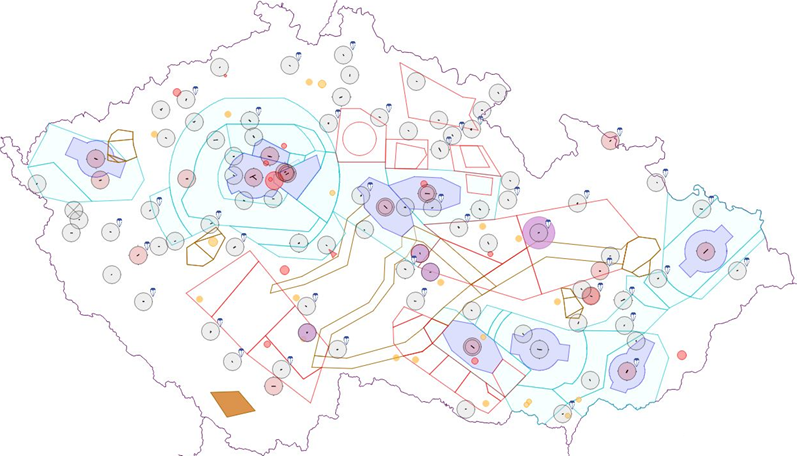
\includegraphics[width=0.75\textwidth]{\FIGDIR/TE057RestrictedAirspaceMap}
    \caption{Example situation in Czech Republic airspace.}
    \label{fig:exampleSituationCzechAirspace}
\end{figure}

\begin{note}
    The most of marked zones are restricted for the RPAS/UAS systems. To integrate RPAS/UAS systems it is necessary to make them compliant with manned aviation regulations and requirements. The impact of RPAS/UAS system failures on human body \cite{authority2013human} and \emph{civil airplanes} \cite{weibel2004safety} outlines future integration requirements.
\end{note}

\paragraph{Aircraft Categorization:} The aircraft categorization for \emph{avoidance priority} is defined in ICAO Annex 2. \cite{icaoAnnex2} also known as \emph{aviation classes for immediate avoidance}. This categorization is based on maneuverability:

\begin{enumerate}
    \item \emph{Manned aviation in distress} - any kind of manned aviation in distress has the highest priority in avoidance.
    
    \item \emph{Balloons} - having only limited vertical maneuverability, impaired by any wind impact significantly, the balloons are avoided by any capable maned aviation.
    
    \item \emph{Gliders} - absence of propulsion impairs vertical avoidance capabilities.
    
    \item \emph{Air fuelling and towing} - dependable load impairs maneuvering capability.
    
    \item \emph{Airships} - limited cruising speed turning angles impairs overall avoidance performance.
    
    \item \emph{Other Manned aviation with propulsion} - normal maneuverability, capable of horizontal and vertical separation
\end{enumerate}

\begin{note}
    This categorization is based on airspace attendant maneuverability    
\end{note}

\noindent There is also supplemental categorization based on operational approach speed (for manned aviation only) \cite{doc20068168} going like follow:
\begin{enumerate}
    \item[\textbf{Class A}] \emph{Small single engine} - cruising speed (100 - 110 knots), runway approach speed (70 - 110 knots).
    
    \item[\textbf{Class B}] \emph{Small multi-engine} - cruising speed (130 - 150 knots), runway approach speed (85 - 130 knots).
    
    \item[\textbf{Class C}] \emph{Airline jet}- cruising speed (160 - 240 knots), runway approach speed (115 - 160 knots).
    
    \item[\textbf{Class D}] \emph{Large jet/military jet}- cruising speed (185 - 265 knots), runway approach speed (130 - 185 knots).
    
    \item[\textbf{Class E}] \emph{Special military}- cruising speed (230 - 275 knots), runway approach speed (155 - 230 knots).
\end{enumerate}

\begin{note}
    The \emph{differences} between cruising speed/runway approach speed are not significant (in terms of ratio). The speed does not impact maneuverability as much as propulsion type and steering elements.
\end{note}